\section{Umsetzungskonzept}
Hier sag ich was ich machen werde

\subsection{Use Case}

Hier Bezug auf Motivation für Energiebranche nehmen und anschließend den Geschftsprotess erläutern.

\subsubsection{Geschäftsprozess}

\subsubsection{Anforderungen}
Anforderungen wie predictive Maintenance und Bezug auf RAMI 4.0.
\subsection{Systementwurf}
Systementwurf: Hier mein angepasstes Architekturmodell -> konkretes Architekturmodell mit Sensoren, Edge Device (RPI), SCP (CF) mit Leo IoT Services; AWS SNS mit API-Schnittstellen

\subsubsection{Systemarchitektur}
\begin{figure}[H]
    \centering
    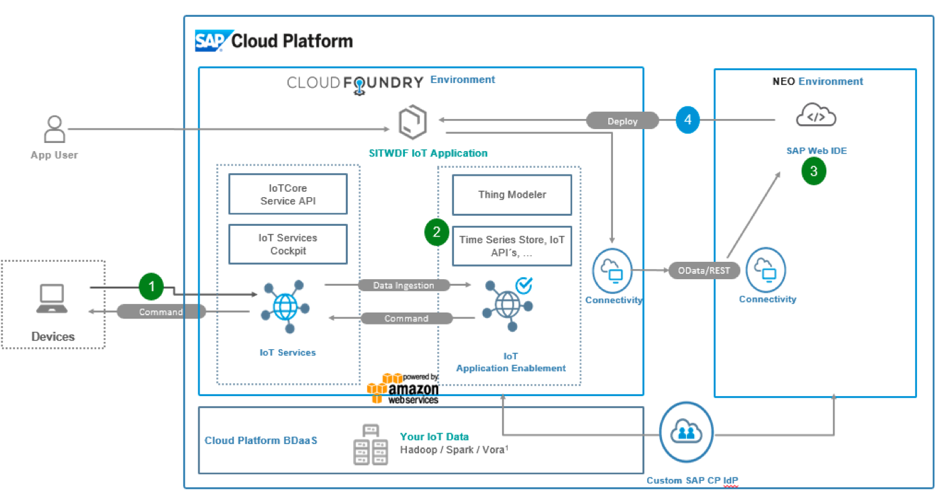
\includegraphics[width=1.0\linewidth]{pictures/sap_architecture}
    \caption[Referenzarchitektur von SAP]{Architektur von SAP \citep{Ganz2019}}
    \label{fig:filename_without_extension}
\end{figure}


\subsubsection{REST}

\subsubsection{Edge-Processing}

\subsubsection{Destinations}
Destinations: Warum braucht man Destinations und welche man benötigt (SNS),  wenn man kommunizieren will mit
Externe Services wie AWS SNS
Interne Kommunikation der SCP CF und NEO
Communication zwischen Cloud Services AWS SNS und SAP Leonardo

\subsubsection{Message Processing}
Leonardo IoT, SQL Kafka: Ich hab Leonardo IoT benutzt (in prototype erwähnen)

\subsubsection{Sicherheit}
OAuth, SSL/TLS, SAML 2.0: erklären, was SAP und AWS auch eventuell haben

\subsection{Prototyp}
Angewandtes/angepasstes System-Modell
pro Schritt benutztes Sicherheitstechnologie erklären/erwähnen

\subsubsection{Anbindung der Sensoren an das Edge-Gerät}

\subsubsection{Geräteverwaltung}
mit SAP Cloud Platform Internet of Things und Device Model hier erstellen und als Bild einfügen und außerdem
zunächst auf Tenants und User eingehen und Einrichtungs des Services generell erklären mit eventuell den Message Processings
und Gateways etc

\subsubsection{Einrichtung der Gateway-Edge}

\subsubsection{Senden der Daten an die Cloud}

\subsubsection{Erstellen des digitalen Zwillings}

\subsubsection{Visualisierung mit einer UI5-Applikation}

\subsubsection{Benachrichtigung mit AWS SNS-Server}

\subsubsection{Events generieren mit NodeJs}

\newpage
